	\subsection{Virtual machine taxonomy by \textit{Smith and Nair}}

	\begin{figure}[H]
		\centering
		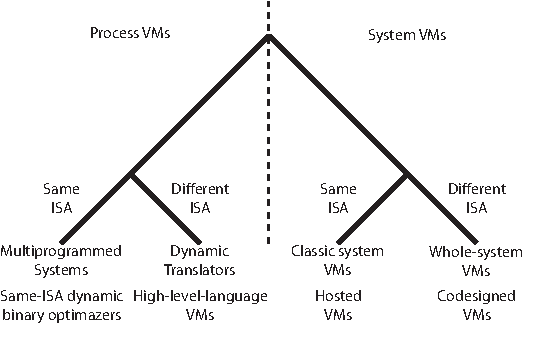
\includegraphics[width=8cm]{images/Smith2005.pdf}
		\vspace{-0.2cm}
		\caption{Virtual machine taxonomy proposed by Smith and Nair in 2005 \cite{Smith2005}.}
		\label{fig:VMTaxonomySmithNair2005}
	\end{figure}
	
	In \textit{Smith} and \textit{Nair}'s study of 2005 \cite {Smith2005}, a taxonomy was presented that its objective was to classify the virtualization technologies into two large groups, such as, \textit{Process VMs} and \textit{System VMs}, see Figure \ref{fig:VMTaxonomySmithNair2005}. 
	
	%LESR - new
	 In general, it could be pointed out that the first level of division (Process vs. System) is about the level of virtualization but of coarser grain than that shown in the \textit{Chiueh's} study \cite{Chiueh2005}. The second level of decomposition refers to whether the virtual machine either Process or System is different from the underlying physical machine or not. 
    
    %JNM 
    System VMs contain an operating system and Process VMs instead access an underlying OS through an Application Binary Interface (ABI) or at the API level. In turn, each category is divided according to the execution or not of ISA simulations, giving rise to various subcategories which are explained below.
	
    %JNM - you could point out that Process vs System is about the level of virtualization but coarser grain than Chiueh2005 
    
    %JNM the second level of decomposition is about whether the virtual machine is different than the underlying physical machine or not
    
    %LESR - see above the new paragraph

	\subsubsection{Process VMs}
	
	The process VMs provide an environment in the ABI interface or at the API level. 
	It is called a multiprogrammed system when it uses the same ISA; otherwise, they are called dynamic emulators and binary translators. 
	The subcategories of the process virtual machines are described below: 
	
	\textbf{Multiprogrammed systems} reference the operating systems that implement multiprogramming through the management of timeshare access to the underlying hardware resources available. These systems use the same ISA and have the ability to handle multiple user processes "simultaneously." The operating system delivers an individual VM for each user process that runs concurrently. One implementation in this context are the \textit{Same-ISA dynamic binary optimizers} using the same ISA from the host system. Furthermore, these translators can make optimized translations of the code, an example of this technology is the Dynamo project \cite{Bala2011}. 
	
	\textbf{Dynamic translators} uses process VMs to support compiled binary programs for an ISA different from the underlying hardware. This implies executing an emulation effort performed through interpretation, which can be relatively slow. This situation can be compensated for through the \textit{dynamic binary translation} when a software cache is implemented to deal with the inherent overload of the binary translation. Examples of this implementation are the VMs of \textit{High-level languages} (HLL)  such as JVM \cite{Lindholm1997} or Microsoft .NET CLI Framework \cite{Fisher2006, Thai2003}.

	\subsubsection{System VMs}
	
	These are characterized by hosting one or several complete and independent operating systems, running simultaneously on the same hardware of the host computer, as a result of the intermediation performed by the VMM. The subcategories of the system VMs are described below:
	
%	\begin{itemize}
	
%		\item \textbf{Classic system VMs} use the VMM and executes it directly on the bare hardware, that is to say, without the presence of an underlying operating system. The VMM  has real access to hardware resources and serves as an intermediary between the guest operating systems and the hardware itself. The VMs in this case are called \textit{Hosted VMs}.
		
%		\item \textbf{Whole-system VMs} provide virtualization of a complete environment, but unlike the previous category, guest systems use an ISA different from the one used in the underlying hardware. The VMs in this case are called \textit{Codesigned VMs}.
%	\end{itemize}

	\textbf{Classic system VMs} use the VMM and executes it directly on the bare hardware, that is to say, without the presence of an underlying operating system. The VMM  has real access to hardware resources and serves as an intermediary between the guest operating systems and the hardware itself. The VMs in this case are called \textit{Hosted VMs}.
		
	\textbf{Whole-system VMs} provide virtualization of a complete environment, but unlike the previous category, guest systems use an ISA different from the one used in the underlying hardware. The VMs in this case are called \textit{Codesigned VMs}.


	%JNM considered as a determinant?
	%LESR I changed "determinant" by "an important base"
	
	\textit{Smith} and \textit{Nair}'s study \cite{Smith2005} can be considered as an important base when classifying virtualization technologies in those that provide a virtual environment for a complete system or processes. However, this work does not contemplate what is established by \textit{Chiueh} \cite{Chiueh2005}, with regards to the levels of abstraction. Another important aspect is that this classification model does not have a high degree of detail, and in contrast, it uses a very general description level without even including particular technologies. It is important to consider that this study was carried out in 2005 and does not include technologies developed  subsequently.
	
